\documentclass{beamer}

\mode<presentation>
\usetheme{Pittsburgh}
\usecolortheme{whale}
\setbeamertemplate{section in toc}{\inserttocsectionnumber.~\inserttocsection}
\setbeamertemplate{subsection in toc}[subsections numbered]
\setbeamertemplate{enumerate items}[default]
\setbeamerfont{caption}{size=\tiny}
\beamertemplatenavigationsymbolsempty{}

\newcommand{\nofootline}{\setbeamertemplate{footline}{}}
\newcommand{\mainfootline}{
  \setbeamertemplate{footline}{
  \hspace*{\fill}
    \insertframenumber{}/\inserttotalframenumber{}
    \hspace*{\fill}
    \vspace{2mm}
  }
}

\usepackage[utf8]{inputenc}
\usepackage[T1]{fontenc}
\usepackage[american]{babel}
\usepackage{cmbright}
\usepackage[scaled=0.85]{beramono}
\usepackage{multimedia}
\usepackage{hyperref}
\usepackage{graphicx}
\usepackage{tikz}
\usepackage{silence}
\usepackage{csquotes}
\usepackage[backend=biber]{biblatex}
\bibliography{/Users/rodrigo/Library/texmf/tex/latex/reference.bib}
\WarningFilter{biblatex}{Patching footnotes failed}
\DeclareFieldFormat*{citetitle}{#1}
\DeclareFieldFormat*{title}{#1}

\graphicspath{
  {img/}
  {/Users/rodrigo/Documents/TUe/thesis/latex/reference/book/Fastl2007Psychoacoustics/img/}
  {/Users/rodrigo/Documents/TUe/thesis/latex/thesis/chapter/img/}
  {/Users/rodrigo/Documents/TUe/thesis/latex/topic/fluctuation_strength/experiment/img/}
  {/Users/rodrigo/Documents/TUe/thesis/latex/topic/fluctuation_strength/model/data_fitting/img/}
}

% ******************************************************************************
% Tikz
% ******************************************************************************

\usetikzlibrary{calc,trees,positioning,arrows,chains,shapes.geometric,%
    decorations.pathreplacing,decorations.pathmorphing,shapes,%
    matrix,shapes.symbols}

\tikzset{
  blockbig/.style={
    rectangle,
    draw=black, very thick,
    text width=30em,
    minimum height=3em,
    text centered,
    on chain},
  blockmedium/.style={
    rectangle,
    draw=black, very thick,
    text width=25em,
    minimum height=3em,
    text centered,
    on chain},
  blockmediumsmall/.style={
    rectangle,
    draw=black, very thick,
    text width=15em,
    minimum height=3em,
    text centered,
    on chain},
  blocksmall/.style={
    rectangle,
    draw=black, very thick,
    text width=10em,
    minimum height=3em,
    text centered},
  blocktiny/.style={
    rectangle,
    draw=black, very thick,
    text width=5em,
    minimum height=3em,
    text centered},
  every join/.style={thick},
}

\tikzstyle{line}=[draw,thick]
\tikzstyle{arrow}=[draw,thick,>=latex,->]

\title{Modeling the Sensation of Fluctuation Strength}
\author{Rodrigo García León
  \texorpdfstring{\\ M.Sc Student Human-Technology Interaction
  \\ \texttt{r.garcia.leon@student.tue.nl}}{}}
\institute{Department of Industrial Engineering \& Innovation Sciences
  \texorpdfstring{\\Eindhoven University of Technology}{}}
\date{December 8, 2015}

\newcommand{\playbutton}{\raisebox{-1ex}{\hbox%
  {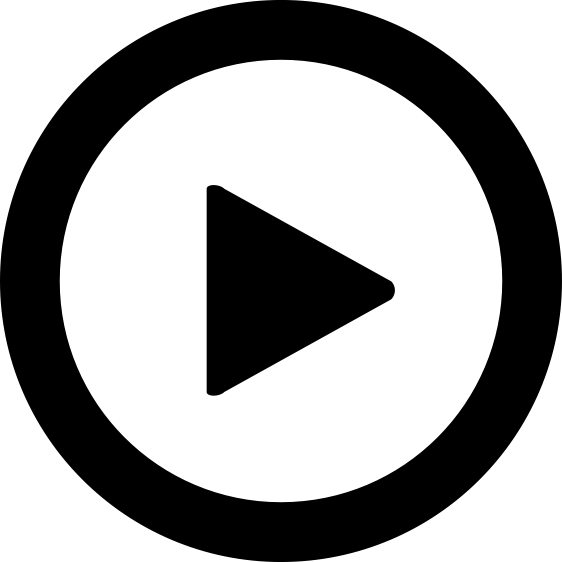
\includegraphics[height=18pt]{play}}}}
\newcommand{\addsound}[1]{
  \movie[label=#1]{}{snd/#1.wav}
  \hyperlinkmovie{#1}{\playbutton}
}
\newcommand{\addcite}[1]{%
  \citeauthor{#1}
  (\citeyear{#1}),
  \citetitle{#1}
}
\newcommand{\addroughnessmodel}{%
  \resizebox{!}{7.5cm}{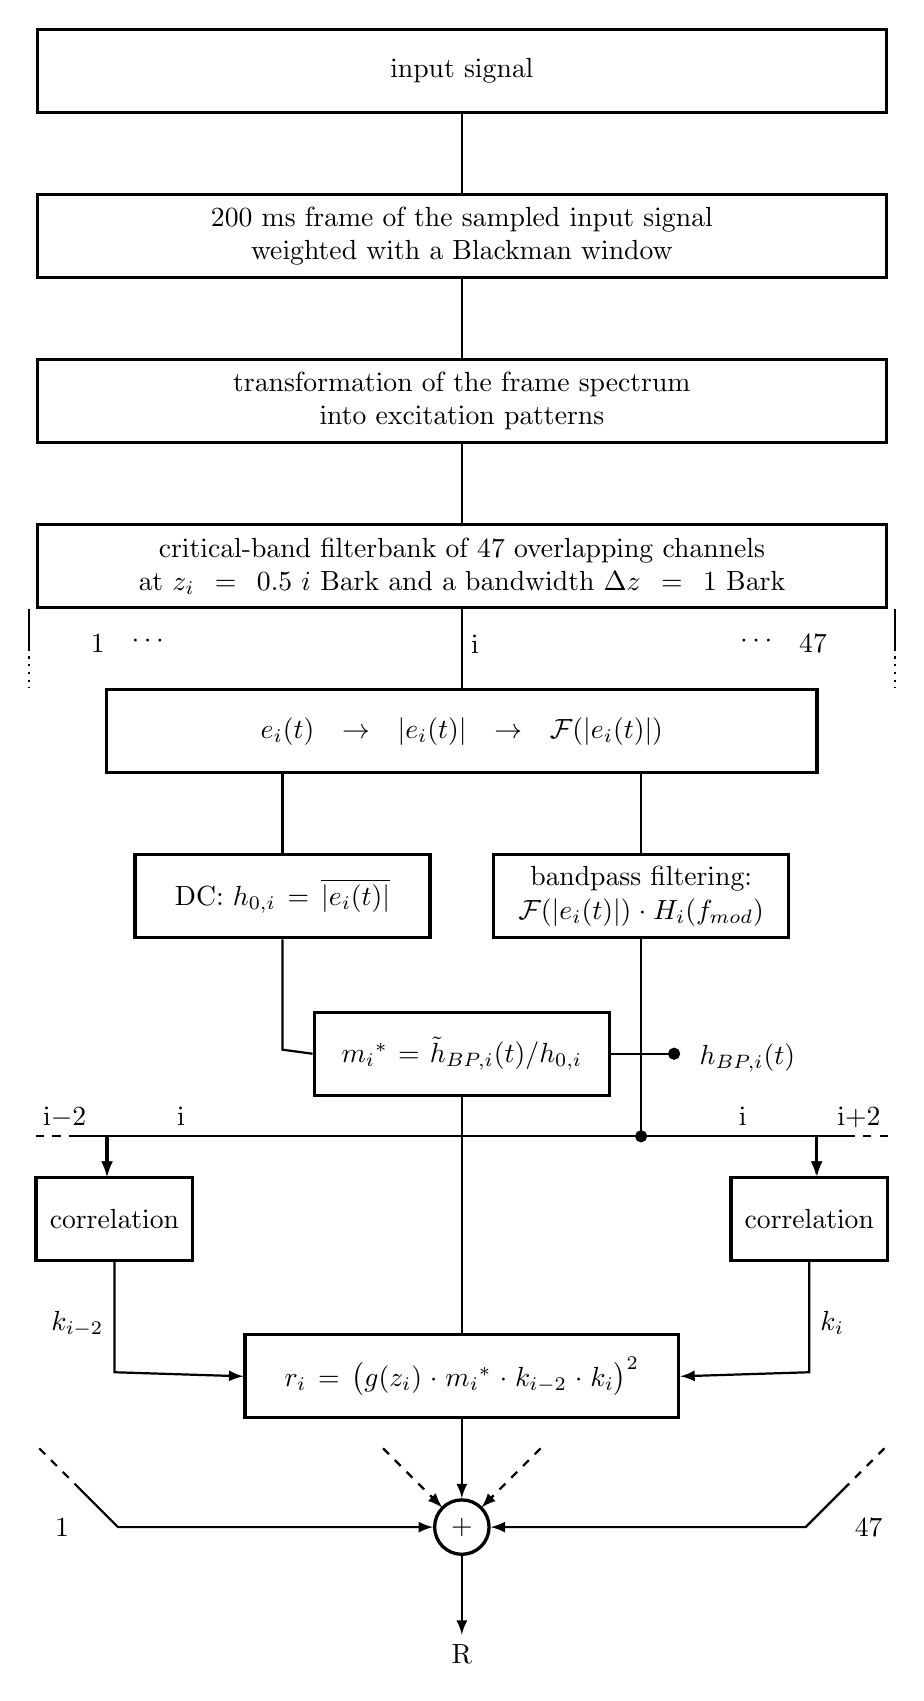
\begin{tikzpicture}
  [node distance=1cm,
  start chain=going below]

  \node[blockbig, join](input)
    {input signal};
  \node[blockbig, join](window)
    {200 ms frame of the sampled input signal\\%
    weighted with a Blackman window};
  \node[blockbig, join](patterns)
    {transformation of the frame spectrum\\into excitation patterns};
  \node[blockbig, join](filterbank)
    {critical-band filterbank of 47 overlapping channels\\%
    at $z_i = 0.5\ i$ Bark and a bandwidth $\Delta z = 1$ Bark};
  \node[blockmedium, join](fourier)
    {$e_{i}(t)\to|e_{i}(t)|\to\mathcal{F}(|e_{i}(t)|)$};
  \node[blocksmall, below left=1cm and -41.5mm of fourier](dc)
    {DC: $h_{0,i}=\overline{|e_{i}(t)|}$};
  \node[blocksmall, below right=1cm and -41.5mm of fourier](filter)
    {bandpass filtering:\\ $\mathcal{F}(|e_{i}(t)|) \cdot H_{i}(f_{mod})$};
  \node[blocksmall, below=3cm of fourier](m*)
    {${m_i}^* = \tilde{h}_{BP,i}(t)/h_{0,i}$};
  \node[blocktiny, below left=1cm and 15mm of m*](correlation_left)
    {correlation};
  \node[blocktiny, below right=1cm and 15mm of m*](correlation_right)
    {correlation};
  \node[blockmediumsmall, below=3cm of m*](ri)
    {$r_i = \big(g(z_i) \cdot {m_i}^* \cdot k_{i-2} \cdot k_i \big)^2$};
  \node[circle, draw=black, very thick, on chain](sum){+};
  \node[on chain](R){R};

  \node[below left=2mm and -5.75cm of filterbank](i){i};
  \node[below left=2mm and -1cm of filterbank](k1){1};
  \node[below left=2mm and -1.75cm of filterbank](d1){$\cdots$};
  \node[below right=2mm and -1.25cm of filterbank](k47){47};
  \node[below right=2mm and -2cm of filterbank](d2){$\cdots$};

  \node[below right=-8mm and 1cm of m*](hbpi){$h_{BP,i}(t)$};
  \node[below left=0cm and 1.5cm of m*](ic2){i};
  \node[below left=0cm and 2.75cm of m*](i-2){i$-$2};
  \node[below right=0cm and 1.5cm of m*](ic1){i};
  \node[below right=0cm and 2.75cm of m*](i+2){i+2};
  \node[below left=5mm and -10mm of correlation_left](ki-2){$k_{i-2}$};
  \node[below right=5mm and -10mm of correlation_right](ki){$k_i$};

  \node[left=4.5cm of sum](c1){1};
  \node[right=4.5cm of sum](c47){47};

  \draw[line] (filterbank.south) +(-5.5,0.0) -- +(-5.5,-0.5);
  \draw[line,dotted] (filterbank.south) +(-5.5,-0.5) -- +(-5.5,-1.0);
  \draw[line] (filterbank.south) +(5.5,0.0) -- +(5.5,-0.5);
  \draw[line,dotted] (filterbank.south) +(5.5,-0.5) -- +(5.5,-1.0);

  \draw[line] (dc.north)--(dc|-fourier.south);
  \draw[line] (filter.north)--(filter|-fourier.south);
  \draw[line] (dc.south) -- +(0.0,-1.4) -- (m*.west);
  \draw[line] (filter.south) -- +(0.0,-2.45);
  \draw[line] (m*.east) -- +(0.8,0.0);
  \draw[line] (m*.south) -- (ri.north);
  \draw[arrow] (m*.south) -- +(0.0,-0.5) -- +(-4.5,-0.5) -- +(-4.5,-1.0);
  \draw[arrow] (m*.south) -- +(0.0,-0.5) -- +(4.5,-0.5) -- +(4.5,-1.0);
  \draw[arrow] (ri.south) -- (sum.north);
  \draw[arrow] (correlation_left.south) -- +(0.0,-1.4) -- (ri.west);
  \draw[arrow] (correlation_right.south) -- +(0.0,-1.4) -- (ri.east);
  \draw[arrow] (sum.south) -- (R.north);

  \draw[line,dashed] (sum.west) +(-5.0,1.0) -- +(-4.5,0.5);
  \draw[arrow] (sum.west) +(-4.5,0.5) -- +(-4.0,0.0) -- (sum.west);
  \draw[line,dashed] (sum.east) +(5.0,1.0) -- +(4.5,0.5);
  \draw[arrow] (sum.east) +(4.5,0.5) -- +(4.0,0.0) -- (sum.east);

  \draw[arrow] (correlation_left.north) +(-0.5,0.5) -- +(-0.1,0.5) --
    +(-0.1,0.0);
  \draw[line,dashed] (correlation_left.north) +(-1.0,0.5) -- +(-0.5,0.5);
  \draw[arrow] (correlation_right.north) +(0.5,0.5) -- +(0.1,0.5) --
    +(0.1,0.0);
  \draw[line,dashed] (correlation_right.north) +(1.0,0.5) -- +(0.5,0.5);

  \draw[arrow,dashed] (sum) +(-1.0,1.0) -- +(-0.25,0.25);
  \draw[arrow,dashed] (sum) +(1.0,1.0) -- +(0.25,0.25);

  \filldraw[black] (m*.east) +(0.8,0.0) circle (2pt);
  \filldraw[black] (filter.south) +(0.0,-2.5) circle (2pt);

\end{tikzpicture}
}
}
\newcommand{\addroughnessnode}{%
  \node[anchor=south west,inner sep=0] at (5.5mm,1mm) {
    \addroughnessmodel{}
  };
}

\AtBeginSection[] {
  {
    \nofootline{}
    \begin{frame}
      \frametitle{Outline}
      \tableofcontents[currentsection]
    \end{frame}
  }
  \addtocounter{framenumber}{-1}
}

\mainfootline{}

\begin{document}

{\nofootline{} \frame{\titlepage}}

\section*{Outline}
{
  \nofootline{}
  \begin{frame}
    \frametitle{Outline}
    \tableofcontents
  \end{frame}
}

\section{Introduction}

\setcounter{framenumber}{0}

\subsection{Perceptual Attributes}
\begin{frame}
  \frametitle{Perceptual Attributes}
  \begin{itemize}
    \item Discernible dimensions into which an auditory event can be decomposed
    \pause{}
    \item Derived from the physical characteristics of sounds (frequency, sound
      pressure level, etc.)
    \pause{}
    \item Examples of them are: loudness, sharpness, roughness, fluctuation
      strength; among others.
    \pause{}
    \item Allow to understand auditory events from a perceptual point of view
  \end{itemize}
\end{frame}

\subsection{Fluctuation Strength}
\begin{frame}
  \frametitle{Fluctuation Strength}
  \begin{itemize}
    \item Sensation that arises from modulated sounds with a slowly varying
      envelope (i.e., a modulation frequency $f_m < 20$ Hz)
    \pause{}
    \item Envelope fluctuation can be amplitude-modulated (AM) or
      frequency-modulated (FM)
  \end{itemize}

  \pause{}

  \begin{columns}
    \begin{column}{0.175\textwidth}
      \hbox{\hbox to 12mm{AM tone} \addsound{am}} \\
      \medskip
      { \scriptsize
        $f_m = 4$ [Hz] \\ $f_c = 1$ [kHz] \\
        SPL = 70 [dB] \\ $m_d = 40$ [dB] \\}
    \end{column}
    \begin{column}{0.175\textwidth}
      \includegraphics[height=0.25\textheight]{am_time}
    \end{column}
    \begin{column}{0.175\textwidth}
      \includegraphics[height=0.25\textheight]{am_frequency}
    \end{column}
  \end{columns}

  \pause{}

  \vspace{2mm}

  \begin{columns}
    \begin{column}{0.175\textwidth}
      \hbox{\hbox to 12mm{FM tone} \addsound{fm}} \\
      \medskip
      { \scriptsize
        $f_m = 4$ [Hz] \\ $f_c = 1.5$ [kHz] \\
        SPL = 70 [dB] \\ $d_f = 700$ [Hz] \\}
    \end{column}
    \begin{column}{0.175\textwidth}
      \includegraphics[height=0.25\textheight]{fm_time}
    \end{column}
    \begin{column}{0.175\textwidth}
      \includegraphics[height=0.25\textheight]{fm_frequency}
    \end{column}
  \end{columns}
\end{frame}

\begin{frame}
  \frametitle{Fluctuation Strength and Roughness}
  \begin{itemize}
    \item Above $f_m > 20$ Hz the fluctuation strength sensation diminishes
      and the roughness sensation begins to take effect
  \end{itemize}

  \pause{}

  \begin{columns}
    \begin{column}{0.175\textwidth}
      \hbox{\hbox to 24mm{Fluctuating tone} \addsound{am}} \\
      \medskip
      { \scriptsize
        $f_m = 4$ [Hz] \\ $f_c = 1$ [kHz] \\
        SPL = 70 [dB] \\ $m_d = 40$ [dB] \\}
    \end{column}
    \begin{column}{0.175\textwidth}
      \includegraphics[height=0.25\textheight]{am_time}
    \end{column}
    \begin{column}{0.175\textwidth}
      \includegraphics[height=0.25\textheight]{am_frequency}
    \end{column}
  \end{columns}

  \pause{}

  \vspace{2mm}

  \begin{columns}
    \begin{column}{0.175\textwidth}
      \hbox{\hbox to 16mm{Rough tone} \addsound{rough}} \\
      \medskip
      { \scriptsize
        $f_m = 70$ [Hz] \\ $f_c = 1$ [kHz] \\
        SPL = 70 [dB] \\ $m_d = 40$ [dB] \\}
    \end{column}
    \begin{column}{0.175\textwidth}
      \includegraphics[height=0.25\textheight]{rough_time}
    \end{column}
    \begin{column}{0.175\textwidth}
      \includegraphics[height=0.25\textheight]{rough_frequency}
    \end{column}
  \end{columns}
\end{frame}

\begin{frame}
  \frametitle{Band-pass Characteristic}
  \begin{figure}
    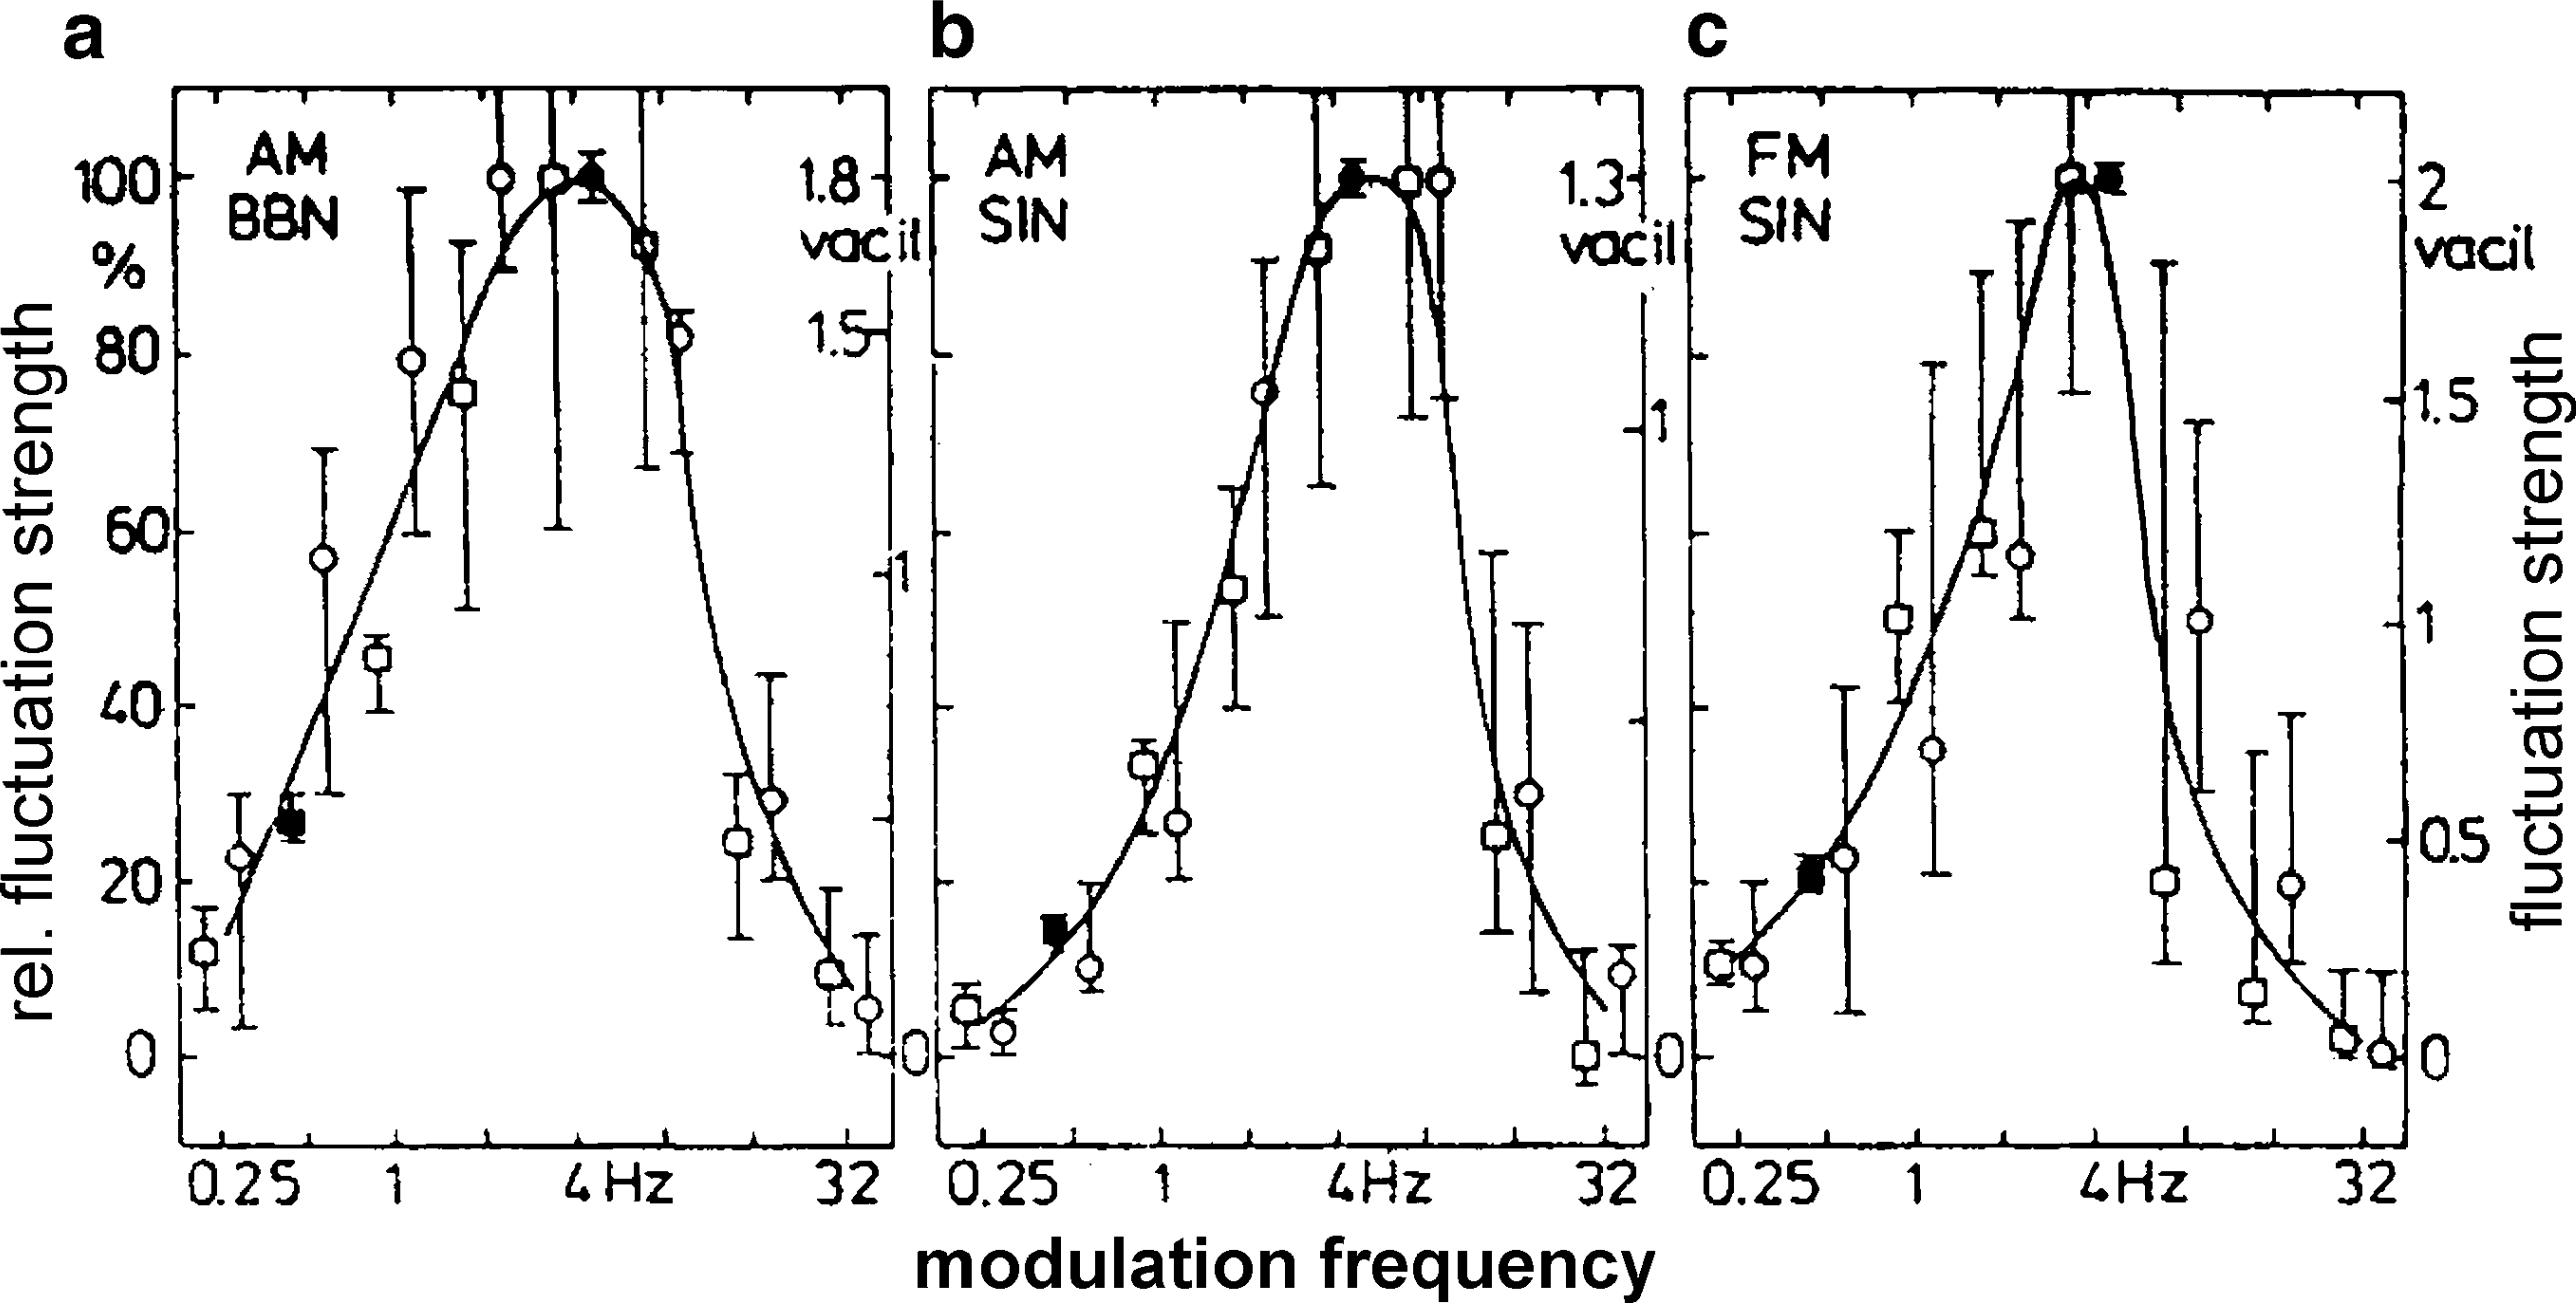
\includegraphics[width=\textwidth]{FluctuationStrengthVsModulationFrequency}
    \caption{Fluctuation strength as a function of modulation frequency for: (a)
      amplitude-modulated broad-band noise, (b) amplitude-modulated tones and
      (c) frequency-modulated tones; as presented by
      \addcite{Fastl2007Psychoacoustics}}
  \end{figure}
\end{frame}

\subsection{Current Research}
\begin{frame}
  \frametitle{Importance}
  \begin{itemize}
    \item Possible relation with the speech system
    \pause{}
    \begin{itemize}
      \item Maximum fluctuation strength value occurs around $f_m = 4$ Hz
      \pause{}
      \item Humans beings utter syllables at a rate of 4 syllables per second
    \end{itemize}
    \pause{}
    \item Influences pleasantness of sounds
    \pause{}
    \begin{itemize}
      \item Functionally (alarm signals)
      \pause{}
      \item Musicality (sound quality and naturalness)
    \end{itemize}
  \end{itemize}
\end{frame}

\begin{frame}
  \frametitle{Rationale for Research}
  \begin{itemize}
    \item Methodological issues in past studies
    \pause{}
    \begin{itemize}
      \item Unfamiliarity with fluctuation strength
      \pause{}
      \item Confusion between roughness and fluctuation strength
    \end{itemize}
    \pause{}
    \item To our knowledge, there is no publicly available work when it comes to
      modeling the sensation of fluctuation strength
  \end{itemize}
\end{frame}

\begin{frame}
  \frametitle{Objectives}
  \begin{itemize}
    \item Formulate a clear methodological procedure to eliminate problems
      found in past studies
    \pause{}
    \item Propose a fluctuation strength model
    \pause{}
    \begin{itemize}
      \item Based on existing roughness models
      \pause{}
      \item Adjusted to collected experimental data
    \end{itemize}
  \end{itemize}
\end{frame}

\section{Experimental Design}

\begin{frame}
  \frametitle{General Details}
  \begin{itemize}
    \item Two conditions: AM tones and FM tones
    \pause{}
    \item 24 participants assigned to one of the two conditions
    \pause{}
    \item Two parts
      \begin{enumerate}
        \item Training phase
        \item Experimental phase
      \end{enumerate}
    \pause{}
    \item Duration of approximately 60 minutes
  \end{itemize}
\end{frame}

\subsection{Training Phase}
\begin{frame}[t]
  \frametitle{Training Phase}
  \begin{enumerate}
    \item Comparison between stimuli: five types of stimuli were presented to
      participants (both for AM and FM)
    \pause{}
      \only<2>{
      \begin{itemize}
        \item Pure tone \addsound{training_1}
        \item Tone with low value of fluctuation \addsound{training_2}
        \item Tone with high value of fluctuation \addsound{training_3}
        \item Tone with low value of roughness \addsound{training_4}
        \item Tone with high value of roughness \addsound{training_5}
      \end{itemize}
      }
    \pause{}
    \item Long intervals: two long intervals (AM and FM), composed of stimuli
      with all the values of modulation frequency used in the experiment, were
      presented to the participants
    \pause{}
    \item Test section: composed of 4 trials, designed to familiarize
      participants with the experimental procedure and interface
  \end{enumerate}
\end{frame}

\subsection{Experimental Phase}
\begin{frame}
  \frametitle{Experimental Phase}
  \begin{itemize}
    \item Magnitude estimation procedure
    \pause{}
    \begin{itemize}
      \item Trial composed of a pair, a standard (reference) with a stimulus,
        separated by 800 ms of silence
      \pause{}
      \item Two standards
      \pause{}
      \item Four repetitions per pair
      \pause{}
      \item Pairs presentation was randomized
    \end{itemize}
    \pause{}
    \item Four parametric variations
    \pause{}
    \begin{itemize}
      \item Modulation frequency ($f_m$)
      \pause{}
      \item Center frequency ($f_c$)
      \pause{}
      \item Sound pressure level (SPL)
      \pause{}
      \item Modulation depth ($m_d$) for AM tones;\\Frequency deviation ($d_f$)
        for FM tones
    \end{itemize}
  \end{itemize}
\end{frame}

\begin{frame}
  \frametitle{APEX Software Platform}
  \centering
  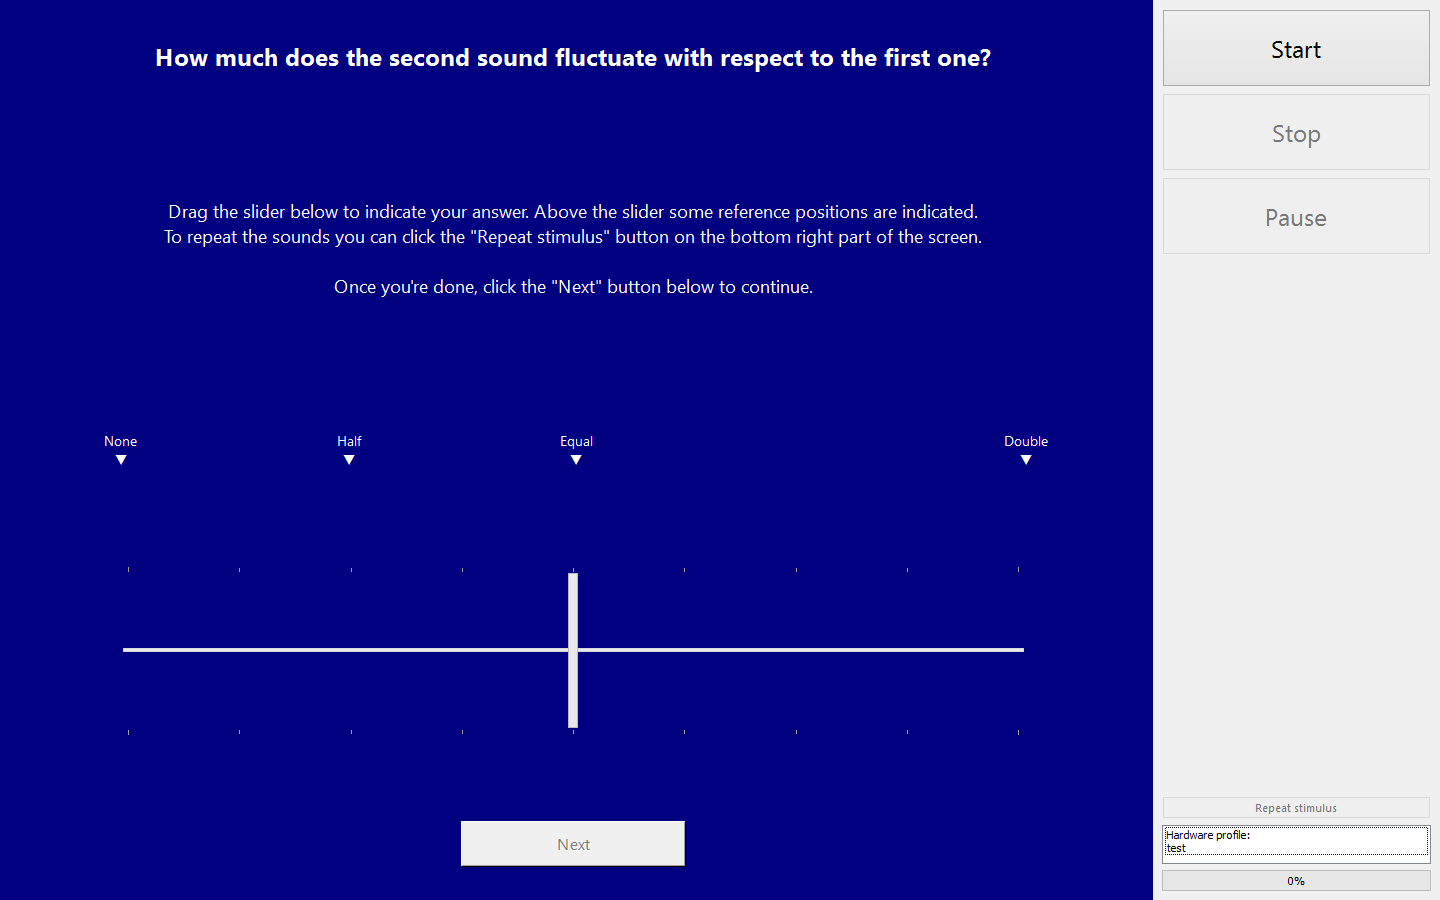
\includegraphics[width=\textwidth]{apex}
  \vspace{2mm}
  \addsound{pair}
\end{frame}

\subsection{Results}
\begin{frame}
  \frametitle{Results --- AM tones, $f_m$}
  \begin{figure}
    \centering
    \begin{minipage}{0.45\textwidth}
      \includegraphics[width=\textwidth]{fastl2007_am-fm}
    \end{minipage}
    \hfill
    \begin{minipage}{0.45\textwidth}
      \includegraphics[width=\textwidth]{AM-fm_all_standards}
    \end{minipage}
    \caption{Relative fluctuation strength as a function of modulation frequency
    for AM tones with center frequency of 1~kHz, sound pressure level of
    70~dB and modulation depth of 40~dB.  The two standards had modulation
    frequencies of 4 and 0.5~Hz. The data points show the median and
    interquartile ranges per standard. The black line represents the mean values
    of the medians of each standard. Left: data adapted from
    \citeauthor[pp.248]{Fastl2007Psychoacoustics}. Right: own results}
  \end{figure}
\end{frame}

\begin{frame}
  \frametitle{Results --- FM tones, $f_c$}
  \begin{figure}
    \centering
    \begin{minipage}{0.45\textwidth}
      \includegraphics[width=\textwidth]{fastl2007_fm-fc}
    \end{minipage}
    \hfill
    \begin{minipage}{0.45\textwidth}
      \includegraphics[width=\textwidth]{FM-fc_all_standards}
    \end{minipage}
    \caption{Relative fluctuation strength as a function of modulation frequency
      for FM tones with center frequency of 1.5~kHz, sound pressure level of
      70~dB and frequency deviation of 700 Hz.  The two standards had modulation
      frequencies of 4 and 0.5~Hz. The data points show the median and
      interquartile ranges per standard. The black line represents the mean values
      of the medians of each standard. Left: data adapted from
      \citeauthor[pp.248]{Fastl2007Psychoacoustics}. Right: own results}
  \end{figure}
\end{frame}

\section{Model Development}

\begin{frame}
  \frametitle{Roughness Model}
  \begin{columns}
    \begin{column}{0.5\textwidth}
      \begin{itemize}
        \item<1-> Presented by \addcite{daniel1997psychoacoustical}
        \item<2-> Composed of three stages
        \begin{enumerate}
          \item<3-> Peripheral stage
          \item<4-> Modulation depth extraction stage
          \item<5-> Specific roughness stage
        \end{enumerate}
        \item<6-> Based on dependence of roughness on modulation depth
        \begin{itemize}
          \item<7-> $R \sim m^p$
        \end{itemize}
      \end{itemize}
    \end{column}
    \begin{column}{0.5\textwidth}
      \centering
      \addroughnessmodel{}
    \end{column}
  \end{columns}
\end{frame}

\subsection{Peripheral Stage}
\begin{frame}
  \frametitle{Peripheral Stage}
  \begin{columns}
    \begin{column}{0.5\textwidth}
    Fluctuation strength model adaptations
      \begin{itemize}
        \item<1-> Separation of input signal into frames
        \item<2-> Outer and middle ear transmission effects
        \item<3-> Critical-band filterbank
      \end{itemize}
    \end{column}
    \begin{column}{0.5\textwidth}
      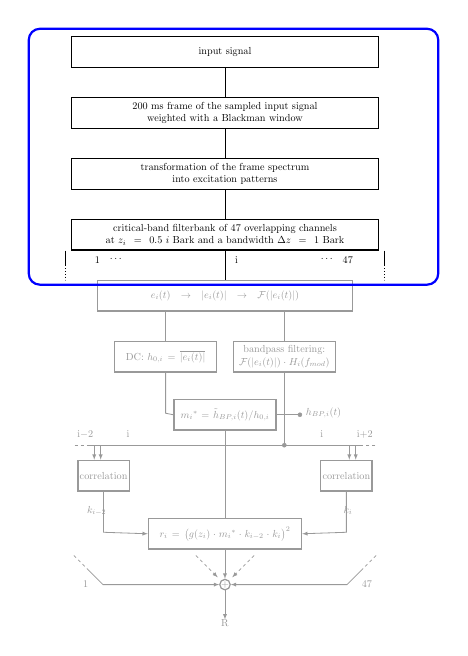
\begin{tikzpicture}
        \addroughnessnode
        \filldraw[fill=white,draw=white,opacity=0.6] (1mm,1mm) rectangle (53mm,45mm);
        \draw[blue,thick,rounded corners] (1mm,44.5mm) rectangle (53mm,77mm);
      \end{tikzpicture}
    \end{column}
  \end{columns}
\end{frame}

\subsection{Modulation Depth Extraction Stage}
\begin{frame}
  \frametitle{Modulation Depth Extraction Stage}
  \begin{columns}
    \begin{column}{0.5\textwidth}
      Fluctuation strength model adaptations
      \begin{itemize}
        \item<1-> Extraction of modulation depth per channel
        \begin{itemize}
          \item<2-> RMS (root mean square) value of bandpass filtered signal
            divided by its mean
          \item<3-> ${m_i}^* = \tilde{h}_{BP,i}(t)/h_{0,i}$
        \end{itemize}
        \item<4-> Bandpass filter using $H_i$ parameter
        \begin{itemize}
          \item<5-> Models the dependence on modulation frequency
        \end{itemize}
      \end{itemize}
    \end{column}
    \begin{column}{0.5\textwidth}
      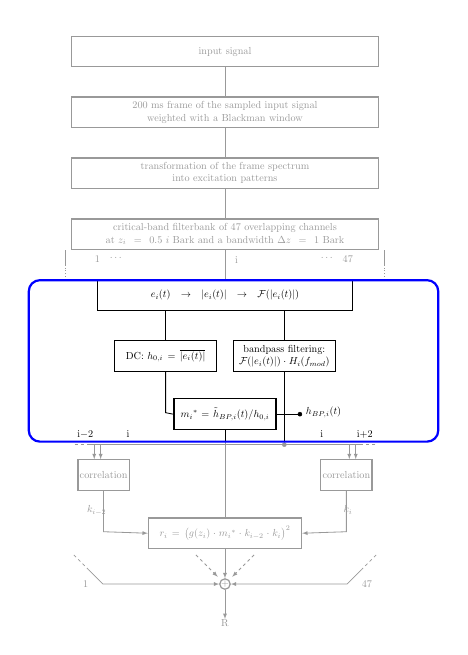
\begin{tikzpicture}
        \addroughnessnode
        \filldraw[fill=white,draw=white,opacity=0.6] (1mm,1mm) rectangle (53mm,24.5mm);
        \filldraw[fill=white,draw=white,opacity=0.6] (1mm,45mm) rectangle (53mm,77mm);
        \draw[blue,thick,rounded corners] (1mm,24.5mm) rectangle (53mm,45mm);
      \end{tikzpicture}
    \end{column}
  \end{columns}
\end{frame}

\begin{frame}
  \frametitle{Roughness of AM Tones}
  \begin{figure}
    \centering
    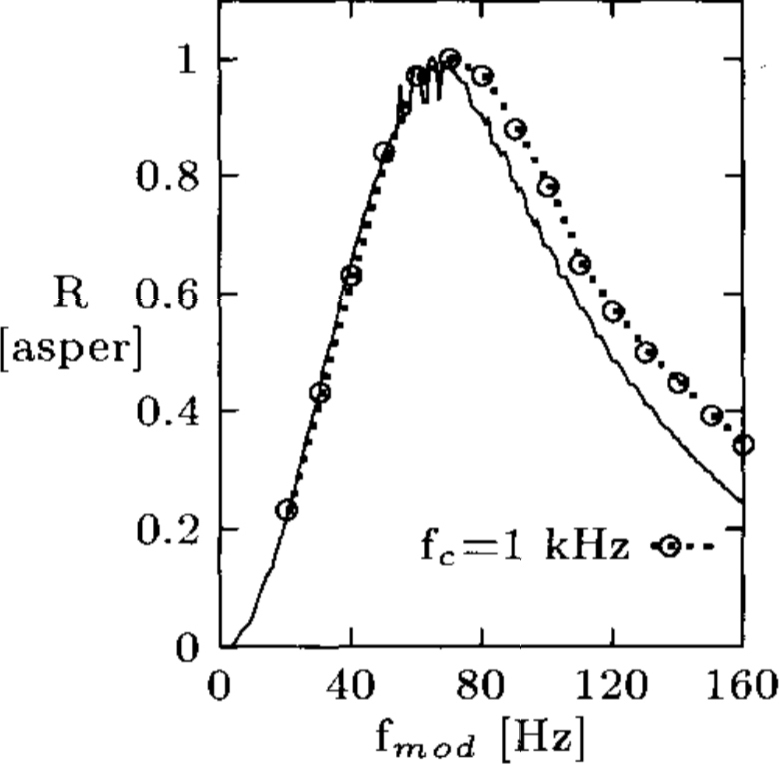
\includegraphics[height=0.5\textheight]{model_roughness}
    \caption{Roughness of AM tones, adapted from
      \addcite{daniel1997psychoacoustical}}
  \end{figure}
\end{frame}

\subsection{Specific Fluctuation Strength Stage}
\begin{frame}
  \frametitle{Specific Fluctuation Strength Stage}
  \begin{columns}
    \begin{column}[T]{0.5\textwidth}
      Fluctuation strength model adaptations
      \begin{itemize}
        \item<only@1-4> Specific fluctuation strength \\
          $f_i = [g(z_i) \cdot {m_i}^* \cdot k_{i-2} \cdot k_i]^2$
        \item<only@2-4> Channel weighting using $g(z_i)$ parameter
        \begin{itemize}
          \item<only@3-4> Models the dependence on center frequency
        \end{itemize}
        \item<only@4> Cross correlations among channels $k_i$
        \item<only@5-> Specific fluctuation strength \\
          $f_i = ({m_i}^{*\prime})^{0.25} \cdot |k_{i-2} \cdot k_i|^{0.375}$
          \only<6>{
          where
          \begin{align}
            {m_i}^{*\prime} &= H({m_i}^{*\prime\prime}) \cdot {m_i}^{*\prime\prime}
            \label{eq:md_transformation_1} \\
            {m_i}^{*\prime\prime} &= {m_i}^* - 0.1
            \label{eq:md_transformation_2}
          \end{align}
          being $H$ the Heaviside step function.
          }
        \item<only@7> Total fluctuation strength \\
          $F = \displaystyle\sum_{i=1}^{47} f_i$
      \end{itemize}
    \end{column}
    \begin{column}[T]{0.5\textwidth}
      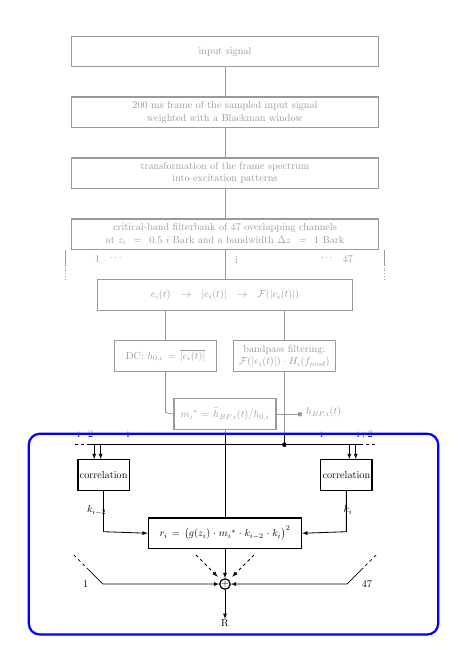
\begin{tikzpicture}
        \addroughnessnode
        \filldraw[fill=white,draw=white,opacity=0.6] (1mm,25.5mm) rectangle (53mm,77mm);
        \draw[blue,thick,rounded corners] (1mm,0mm) rectangle (53mm,25.5mm);
      \end{tikzpicture}
    \end{column}
  \end{columns}
\end{frame}

\subsection{Results}
\begin{frame}
  \frametitle{Results --- $f_m$}
  \begin{figure}
    \centering
    \begin{minipage}{0.45\textwidth}
      \includegraphics[width=\textwidth]{garcia2015_am-fm}
    \end{minipage}
    \hfill
    \begin{minipage}{0.45\textwidth}
      \includegraphics[width=\textwidth]{garcia2015_fm-fm}
    \end{minipage}
    \caption{Fluctuation strength as a function of modulation frequency for
      AM tones (left) and FM tones (right). The blue dashed line corresponds to
      the mean of the two standards of the experimental data. The black solid
      line corresponds to the output of the model. In the top left corner the
      square root of the sum of the square of the difference between these two
      curves ($\sqrt{\sum r_i^2}$) is shown}
  \end{figure}
\end{frame}
\begin{frame}
  \frametitle{Results --- $f_c$}
  \begin{figure}
    \centering
    \begin{minipage}{0.45\textwidth}
      \includegraphics[width=\textwidth]{garcia2015_am-fc}
    \end{minipage}
    \hfill
    \begin{minipage}{0.45\textwidth}
      \includegraphics[width=\textwidth]{garcia2015_fm-fc}
    \end{minipage}
    \caption{Fluctuation strength as a function of center frequency for
      AM tones (left) and FM tones (right). The blue dashed line corresponds to
      the mean of the two standards of the experimental data. The black solid
      line corresponds to the output of the model. In the top left corner the
      square root of the sum of the square of the difference between these two
      curves ($\sqrt{\sum r_i^2}$) is shown}
  \end{figure}
\end{frame}

\section{Discussion}
\begin{frame}
  \frametitle{Discussion}
  \begin{itemize}
    \item<1-> Training phase helps participants understand the concept of
      fluctuation strength
    \begin{itemize}
      \item<2-> It does not eliminate confusion completely
      \item<3-> Unfamiliarity, forgetfulness, over-thinking
    \end{itemize}
    \item<4-> \citeauthor{Fastl2007Psychoacoustics} data and obtained data are
      qualitatively similar
    \begin{itemize}
      \item<5-> Differences in sensitivity to center frequency and frequency
        spread
    \end{itemize}
    \item<6-> It is possible to adjust \citeauthor{daniel1997psychoacoustical}
      model to the fluctuation strength sensation
    \begin{itemize}
      \item<7-> Model designed specifically for AM tones
      \item<8-> Slow computation due to increased frame size
    \end{itemize}
  \end{itemize}
\end{frame}

\section*{Questions}
{
  \nofootline{}
  \begin{frame}
    \frametitle{Questions}
    \centering
    \vspace*{\fill}
    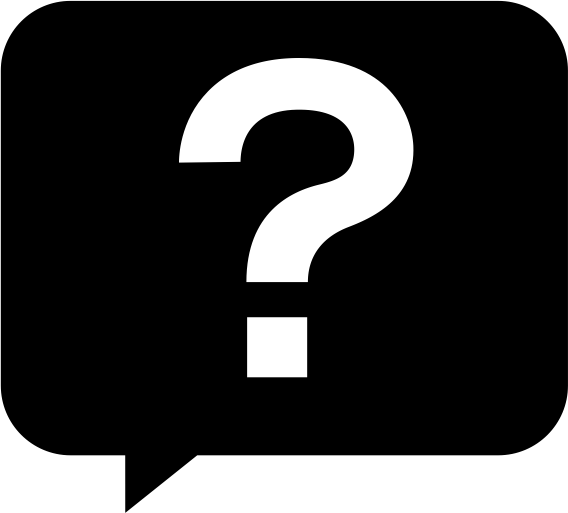
\includegraphics[height=0.6\textheight]{question}
    \vspace*{\fill}
  \end{frame}
}
\addtocounter{framenumber}{-1}

\section*{Credits}
{
  \nofootline{}
  \begin{frame}
    \frametitle{Credits}
    \begin{itemize}
      \item play \playbutton{} by Mike Ashley from Noun Project
      \item question
        \raisebox{-1ex}{\hbox{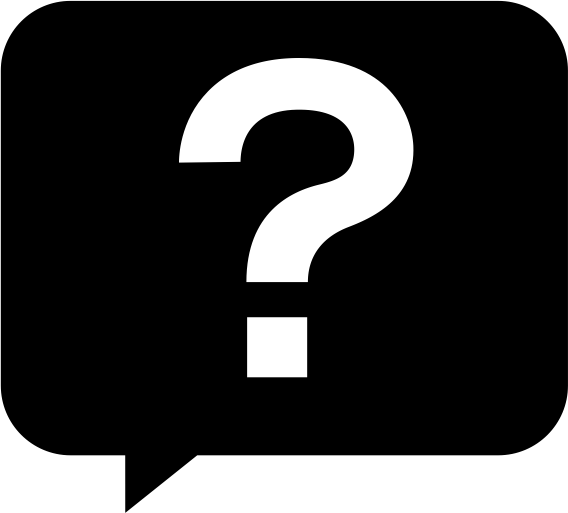
\includegraphics[height=18pt]{question}}} by
        Henry Ryder from Noun Project
    \end{itemize}
  \end{frame}
}
\addtocounter{framenumber}{-1}

\end{document}
